% mainfile: ../../Refinement.tex
To gain more understanding of the \picalc{} we will use \findex[stargazer]{Stargazer}\cite{stargazer}. Stargazer is a visual simulator for \picalc{}. \refLis{pi_visualization_stargazer_code} shows the code of the process $P\define\procres{x}{(\procpar{\proccall{A_1}{x}}{\proccall{B_1}{x}})}$ where: $\procdef{A_1}{y}\define{}\out{y}{{}}.\proccall{A_2}{y}$ and $\procdef{B_1}{z}\define{}\inp{z}{{}}.\proccall{B_2}{z}$ in stargazer syntax.
\lstinputlisting[backgroundcolor=\color{white},caption={stargazer code for the process $P$.},captionpos=b, label={pi_visualization_stargazer_code}]{listings/pi_visualization_stargazer.pi}
\raggedbottom

Stargazer can visualize the reaction $\procres{x}{(\procpar{\proccall{A_1}{x}}{\proccall{B_1}{x}})} \transs{\tau} \procres{x}{(\procpar{\proccall{A_2}{x}}{\proccall{B_2}{x}})}$ as shown in
\refFig{pi_visualization_stargazer_reaction}.
\begin{figure}[H]%
\centering
\subcaptionbox{Before reaction occurrence.}{\fbox{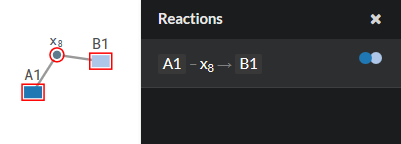
\includegraphics[width=0.45\textwidth]{./images/pi_visualization_stargazer_Before_react.png}}}%
\hfill
\subcaptionbox{After reaction occurrence.}{\fbox{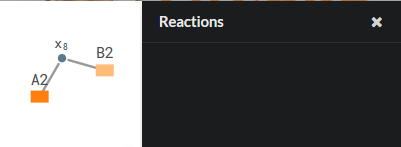
\includegraphics[width=0.45\textwidth]{./images/pi_visualization_stargazer_After_react.png}}}%
\caption{The process $P$ reaction}
\label{pi_visualization_stargazer_reaction}%
\end{figure}